\documentclass[a4paper, 12pt]{article}

%%% Работа с русским языком
\usepackage{cmap}					% поиск в PDF
\usepackage{mathtext} 				% русские буквы в формулах
\usepackage[T2A]{fontenc}			% кодировка
\usepackage[utf8]{inputenc}			% кодировка исходного текста
\usepackage[russian]{babel}	% локализация и переносы

%%% Дополнительная работа с математикой
\usepackage{amsmath,amsfonts,amssymb,amsthm,mathtools} % AMS
\usepackage{icomma} % "Умная" запятая: $0,2$ --- число, $0, 2$ --- перечисление

%% Номера формул
%\mathtoolsset{showonlyrefs=true} % Показывать номера только у тех формул, на которые есть \eqref{} в тексте.
%\usepackage{leqno} % Немуреация формул слева

%% Шрифты
\usepackage{euscript}	 % Шрифт Евклид
\usepackage{mathrsfs} % Красивый матшрифт

%%% Свои команды
\DeclareMathOperator{\sgn}{\mathop{sgn}}

%% Поля
\usepackage[left=2cm,right=2cm,top=2cm,bottom=2cm,bindingoffset=0cm]{geometry}

%% Русские списки
\usepackage{enumitem}
\makeatletter
\AddEnumerateCounter{\asbuk}{\russian@alph}{щ}
\makeatother

%%% Работа с картинками
\usepackage{graphicx}  % Для вставки рисунков
\graphicspath{{images/}{images2/}}  % папки с картинками
\setlength\fboxsep{3pt} % Отступ рамки \fbox{} от рисунка
\setlength\fboxrule{1pt} % Толщина линий рамки \fbox{}
\usepackage{wrapfig} % Обтекание рисунков и таблиц текстом

%%% Работа с таблицами
\usepackage{array,tabularx,tabulary,booktabs} % Дополнительная работа с таблицами
\usepackage{longtable}  % Длинные таблицы
\usepackage{multirow} % Слияние строк в таблице

%% Красная строка
\setlength{\parindent}{2em}

%% Интервалы
\linespread{1}
\usepackage{multirow}

%% TikZ
\usepackage{tikz}
\usetikzlibrary{graphs,graphs.standard}

%% Верхний колонтитул
\usepackage{fancyhdr}
\pagestyle{fancy}

%% Перенос знаков в формулах (по Львовскому)
\newcommand*{\hm}[1]{#1\nobreak\discretionary{}
	{\hbox{$\mathsurround=0pt #1$}}{}}

%% дополнения
\usepackage{float} %Добавляет возможность работы с командой [H] которая улучшает расположение на странице
\usepackage{gensymb} %Красивые градусы
\usepackage{caption} % Пакет для подписей к рисункам, в частности, для работы caption*

% подключаем hyperref (для ссылок внутри  pdf)
\usepackage[unicode, pdftex]{hyperref}

%%% Теоремы
\theoremstyle{plain}                    % Это стиль по умолчанию, его можно не переопределять.
\renewcommand\qedsymbol{$\blacksquare$} % переопределение символа завершения доказательства

\newtheorem{theorem}{Теорема}[section] % Теорема (счетчик по секиям)
\newtheorem{proposition}{Утверждение}[section] % Утверждение (счетчик по секиям)
\newtheorem{definition}{Определение}[section] % Определение (счетчик по секиям)
\newtheorem{corollary}{Следствие}[theorem] % Следстиве (счетчик по теоремам)
\newtheorem{problem}{Задача}[section] % Задача (счетчик по секиям)
\newtheorem*{remark}{Примечание} % Примечание (можно переопределить, как Замечание)
\newtheorem{lemma}{Лемма}[section] % Лемма (счетчик по секиям)

\newtheorem{example}{Пример}[section] % Пример
\newtheorem{counterexample}{Контрпример}[section] % Контрпример

\begin{document}
    \newcommand{\HRule}{\rule{\linewidth}{0.7mm}} % Defines a new command for the horizontal lines, change thickness here
	
	\begin{center}
		\large\textbf{Московский Физико-Технический Институт}\\ % Name of your university/college
		\large\textbf{(государственный университет)}
	
		\vfill
		
		\Large Государственный экзамен по общей физике. Вопрос по выбору.\\[0.5cm] % Preambule of your document title
		
		
		\HRule
		\\[0.4cm]
		{ \huge \bfseries Численное решение временного уравнения Шрёдингера и визуализация физических моделей на его основе.}% Title of your document
		\\[0.4cm] 
		\HRule
		\\[0.5cm]
		
		\ \\
	\textbf{\large Автор:} \\	
	\large Филиппенко Павел Б01-009\\ % Your name and something more, your group num for example
		\vfill
		\hspace*{-0.8 cm}
\includegraphics[width=100 pt]{../images/frkt_logo}\\ % logo of your  company/university/college
		\large Долгопрудный, 2023 % location and year
	\end{center}

\newpage
\setcounter{page}{2}
\fancyfoot[c]{\thepage}
\fancyhead[L] {} % some information in page header
\fancyhead[R]{}

    \tableofcontents{} %содержание
    \newpage

    \section{Постановка задачи}

    В рамках данной работы мы рассмотрим эффект надбарьерного и подбарьерного перехода квантовой частицы.
    Конктретно сконцентриуем внимание на эффекте квантового туннелирования. В практической части работы с помощью
    численного решения временного уравнения Шрёдингера мы смоделируем визуализацию волновой функции. 
    Кроме того мы рассмотрим ее взаимодействие с различными видами потенциальных барьеров и пронаблюдаем зависимости
    различных параметров, полученных теоретическим путем.

    \section{Уравнение Шрёдингера}

    В терминах операторов уравнение Шрёдингера записывается следующим образом

    \begin{equation}
        \hat{H} \psi = E \psi
    \end{equation}

    где $\hat{H}$ -- в данном случае оператор полной энергии (гамильтониан), $E$ -- полная энергия квартовой частицы. Запишем выражение для оператора $\hat{H}$

    \begin{equation}
        \hat{H} = - \frac{\hbar^2}{2m} \Delta + U
    \end{equation}

    где $\Delta$ -- оператор Лапласа, $U$ -- потенциальная энергия. В рамках данной работы мы считаем, что потенциальная энергия
    является функцией чисто координаты, то есть не зависит от вермени. Тогда уравнение Шредингера можно переписать, как
    дифференциальное уравнение второго порядка

    \begin{equation}
        \Delta \psi + \frac{2m}{\hbar^2} (E - U) \psi = 0
    \end{equation}

    Для перехода к более общему случаю -- уравнению, которое описывает волновую функцию $\psi$ во времени заменим в исходном 
    уравнении $E$ на соответствующий оператор. 

    \begin{equation}
        i \hbar \frac{\partial \psi}{\partial t} = \hat{H} \psi
    \end{equation}

    Заметим, что в соответствии с теорией дифференциальных уравнений для нахождения решения 
    для всех моментов времени необходимо единственное начальное решение $\psi(r, 0)$.

    Заметим так же, что оператор $\hat{H}$ не зависит от времени и действует только на функции от координат. Это позволяет
    произвести разделение переменных $r$ и $t$.

    \[ \psi(r, t) = f(t) \phi(r) \]

    Подставляя в уравнение, получим

    \[ i \hbar \psi(r) \frac{df}{dt} = f(t) \hat{H} \phi(r) \]

    \[ i \hbar \frac{1}{f(t)} \frac{df}{dt} = \frac{1}{\phi(r)} \hat{H} \phi(r) \]

    В равенстве левая и правая части зависят от разных переменных, таким образом, чтобы равенство было верным,
    необходимо, чтобы обе части уравнения были постоянными. Обозначим

    \[ i \hbar \frac{1}{f(t)} \frac{df}{dt} = \frac{1}{\phi(r)} \hat{H} \phi(r) = E \]

     Тогда, с одной стороны мы получаем уравнение для стационарного случая

     \[ \hat{H} \phi(r) = E \phi(r) \]

     а с другой стороны решение части, зависящей от времени

     \[ f(t) = const \cdot e^{\frac{-iEt}{\hbar}} \]

     Таким образом, решение временного уравнения записывается следующим образом

     \begin{equation}
         \psi(r, t) = \phi(r) e^{-iEt}
     \end{equation}
    
    \section{Прямоугольный потенциальный барьер}

    Основной задачей в данном разделе будет получение выражения для коэффициентов надбарьерного перехода (в случае
    $E > U$) и подбарьерного перехода (в случае $E < U$).

    При решении подобных задач стандартный способ заключается в составлении уравнений Шрёдингера для различных зон,
    в зависимости от распределения потенциальной энергии, а так же записи граничных условий. Общий вид такого
    стационарного уравнения

    \begin{equation}
        \frac{d^2 \psi}{dx^2} + k^2 \psi = 0
    \end{equation}

    где 

    \begin{equation}
        k^2 = \frac{2m}{\hbar^2} (E - U)
    \end{equation}
    
    Будем обозначать $r$ и $d$ --
    коэффициенты отражения и прохождения по амплитуде соответственно, $R$ и $D$ -- коэффициенты отражения и прохождения
    по энергии. Записывая систему уравнений для различных зон, а так же граничные условия, можно установить выражения для
    коэффициентов $r$ и $d$:

    \begin{equation}
        r = \frac{k_1 - k_2}{k_1 + k_2}
    \end{equation}

    \begin{equation}
        d = \frac{2 k_1}{k_1 + k_2}
    \end{equation}

    Выражения для коэффициентов отражения и прохождения по энергии выводятся с применения понятия плотности потока вероятности

    \begin{equation}
        R = |r|^2
    \end{equation}

    \begin{equation}
        \frac{k_2}{k_1} |d|^2
    \end{equation}

    Подробный вывод данных формул в рамках данной работы мы опустим.

    Рассмотрим некоторые общие соотношения, связывающие амплитудные коэффициенты отражения и пропускания волн де Бройля на
    границе барьера.

    \begin{figure}
        \centering
        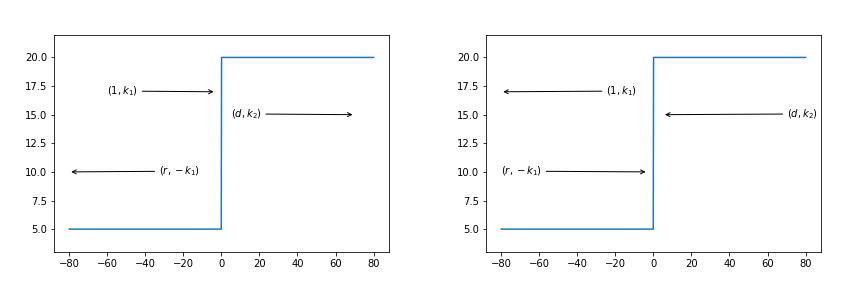
\includegraphics[scale=0.5]{images/StepBarrier.jpg}
        \caption{Волны на границе}
        \label{fig:StepBarrier}
    \end{figure}

    Рассматривая рисунок \ref{fig:StepBarrier} обозначим за $r$, $d$ амплитудные коэффициенты в случае, когда волна 
    распространяется слева направо, и $r'$, $d'$ когда волна распространяется справа налево.
    Утверждается, что если поменять направления всех волн без изменения их амплитуд, то граничные условия не изменятся.
    В любом случае на границе должен выполняться баланс амплитуд прошедших и отраженных волн. Используя это утверждение,
    можно записать

    \begin{equation} \label{eq:r'd'}
        \begin{cases}
            r^2 + dd' = 1 \\
            rd + dr' = 0
        \end{cases}
    \end{equation}

    откуда получаем важноые соотношения $r = -r'$, $\displaystyle d' = \frac{1 - r}{d}$. 
    Мы воспользуемся ими дальше, а сейчас перейдем, наконец, к рассмотрению
    нашей непосредственной задачи.

    \begin{figure}
        \centering
        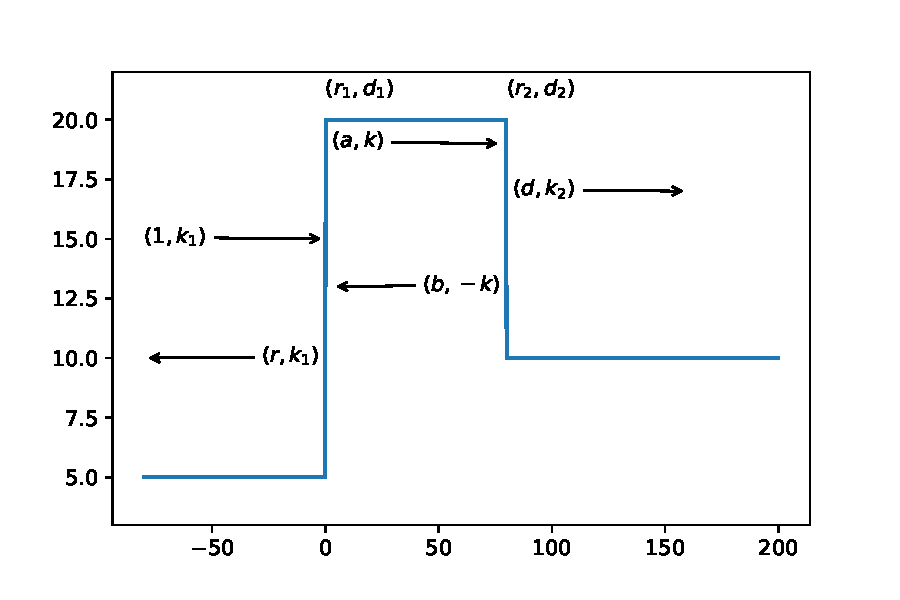
\includegraphics{images/PotentialBarrier.pdf}
        \caption{Прохождение волны через потенциальный барьер}
        \label{fig:PotentialBarrier}
    \end{figure}

    В данном случае, потенциал в пространстве распределен следующим образом

    \begin{equation}
        U(x) = 
        \begin{cases}
            U_1 ~~~ x < 0 \\
            U ~~~ 0 \leq x \leq a \\
            U_2 ~~~ x > a
        \end{cases}
    \end{equation}

    Запишем уравнения Шрёдингера для каждой зоны

    \[ \psi'' + \frac{2m(E - U_1)}{\hbar^2} \psi = 0 \]
    \[ \psi'' + \frac{2m(E - U)}{\hbar^2} \psi = 0 \]
    \[ \psi'' + \frac{2m(E - U_2)}{\hbar^2} \psi = 0 \]
    
    Поскольку мы рассматриваем случай $E < U$ (случай подбарьерного перехода), введем обозначения для коэффициентов $k$

    \[ k_1 = \frac{\sqrt{2m(E - U_1)}}{\hbar} \]
    \[ k = i \alpha = \frac{\sqrt{2m(E - U)}}{\hbar} \]
    \[ k2 = \frac{\sqrt{2m(E - U_2)}}{\hbar} \]
    
    где $\displaystyle \alpha = \frac{\sqrt{2m(U - E)}}{\hbar}$.

    Рассматривая прохождение потенциального барьера конечной ширины $l$ рис \ref{fig:PotentialBarrier}, обозначим
    $r_1$, $d_1$ -- амплитудные коэффициенты на первой границе, $r_2$, $d_2$ -- амплитудные коэффициенты на второй границе.
    При распространении волны в обратном направлении, соответственно $r_1'$, $d_1'$, $r_2'$, $d_2'$. 
    За  $r$ и $d$ обозначим амплитудные коэффициенты при прохождении всего барьера. Тогда, рассматривая волны
    на правой и левой границе, получим

    \[ r = r_1 + d_1 b ~~~ a = d_1 + r_1' b \]
    \[ d e^{ik_2l} = d_2 a e^{ikl} ~~~ b e^{-ikl} = r_2 a e^{ikl} \]
    
    Решая эту систему, и учитывая соотношения \eqref{eq:r'd'} получим выражения для амплитудных коэффицинтов

    \begin{equation}
        r = \frac{r_1 + r_2 e^{2ikl}}{1 + r_1 r_2 e^{2ikl}} ~~~ d = \frac{d_1 d_2 e^{-i(k_2 - k)l}}{1 + r_1 r_2 e^{2ikl}}
    \end{equation}

    Подставляя

    \begin{equation}
        r_1 = \frac{k_1 - k}{k_1 + k} ~~~ d_1 = \frac{2k_1}{k_1 + k}
    \end{equation}

    \begin{equation}
        r_2 = \frac{k - k_2}{k + k_2} ~~~ d_2 = \frac{2k}{k + k_2}
    \end{equation}

    а так же используя выражение 

    \[ D = \frac{k_2}{k_1} |d|^2 = \frac{k_2}{k_1} d d^*  \]

    получим формулу для коэффициента подбарьерного перехода

    \begin{equation}
        D = \frac{16 k_1 k_2 \alpha^2}{(k_1^2 + \alpha^2)(k_2^2 + \alpha^2)(e^{2\alpha l} + e^{-2\alpha l}) + 2(\alpha^2 - k_1 k_2)}
    \end{equation}

    Итак, мы получили общее выражение для подбарьерного перехода. В рамках нашей численной задачи, мы будем рассматривать
    частный случай, при котором $U_1 = U_2 = 0$, $U = U_0$, тогда выражение для $D$ можно легко переписать в терминах 
    энергий

    \begin{equation}
        D = \frac{1}{1 + \frac{U_0^2}{4 E (U_0 - E)}\sinh^2 {k l}}
    \end{equation}

    где $\displaystyle k = \frac{\sqrt{2m (U_0 - E)}}{\hbar}$. Именно это выражение мы будем использовать в качестве
    результата теоретического расчета при исследовании численного решения. 

    Проводя аналогичные рассуждения для ситуации, в которой $E > U$ (надбарьерный переход), для коэффициента прохождения получим
    следующее выражение

    \begin{equation}
        D = \frac{1}{1 + \frac{U_0^2}{4 E (U_0 - E)}\sin^2 {k l}}
    \end{equation}

    где $\displaystyle k = \frac{\sqrt{2m (E - U_0)}}{\hbar}$.

    Довольно интересным оказывается рассмотреть зависимости коэффициентов надбарьерного и подбарьерного перехода в зависимости от
    энергии $E$.

    \begin{figure}
        \centering
        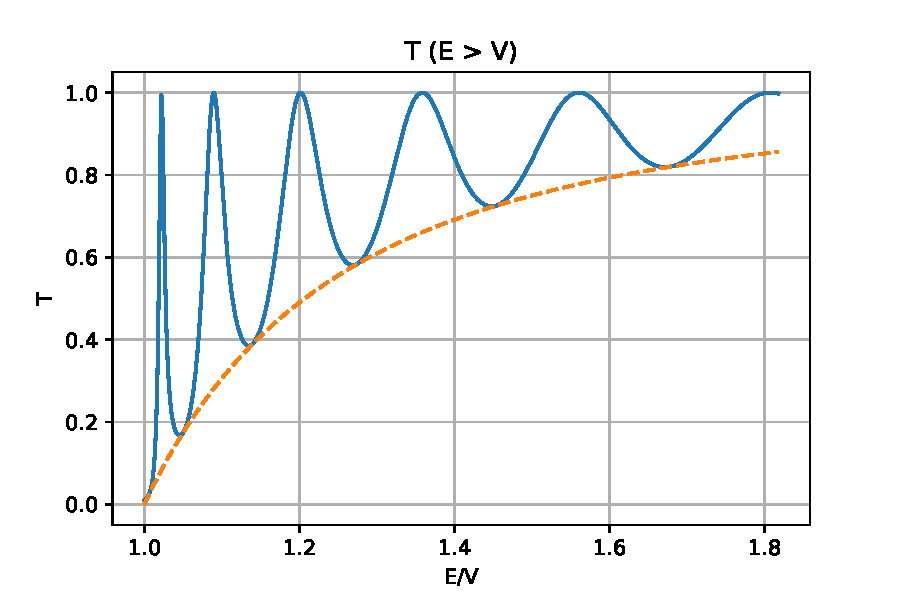
\includegraphics{images/TransmissionPropability1.pdf}
        \caption{Коэффициент надбарьерного перехода}
        \label{fig:TransmissionPropability1}
    \end{figure}

    \begin{figure}
        \centering
        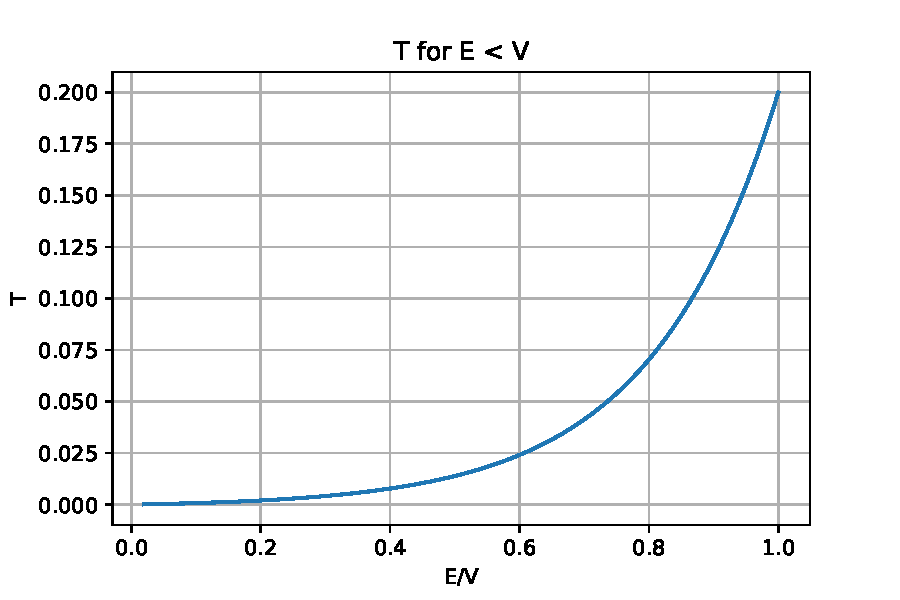
\includegraphics{images/TransmissionPropability2.pdf}
        \caption{Коэффициент подбарьерного перехода}
        \label{fig:TransmissionPropability2}
    \end{figure}

    Рассматривая графики \ref{fig:TransmissionPropability1} и \ref{fig:TransmissionPropability2} можно заметить следующие
    закономерности:

    \begin{enumerate}
        \item Коэффициент надбарьерного перехода не возрастает строго, а осцилирует. Это возникает в силу наличия синуса в 
        знаменателе. Это значит, что частица с более высокой энергией не обязательно имеет большую вероятность преодоления 
        барьера.
        \item Коэффициент подбарьерного перехода монотонно возрастает с увеличением энергии. Это значит, что чем больше
        энергия частицы, тем больше вероятность ее проскочить под барьером.
    \end{enumerate}

    Данные утверждения мы в дальнейшем проверим визуально.
    
    \section{Численное решение уравнения Шрёдингера и создание визуализации}

    \subsection{Численное решение}

    Запишем уравнение Шрёдингера, зависящее от времени

    \begin{equation}
        i \hbar \frac{\partial \psi}{\partial t} = \hat{H} \psi(r, t)
    \end{equation}

    где $\hat{H}$ -- в данном случае оператор полной энергии (гамильтониан). Запишем этот оператор

    \begin{equation}
        \hat{H} = - \frac{\hbar^2}{2m} \Delta + U(r)
    \end{equation}

    где $\Delta$ -- оператор Лапласа. Решение полученного дифференциального уравнения записывается следующим образом

    \begin{equation} \label{eq:solution}
        \psi(r, t) = \exp(-i H t) \psi(r, 0)
    \end{equation}
    
    Перейдем к обсуждению численного решения. Пространственный интервал поделим сеткой на $N$ частей.
    В каждый отдельный момент времени волновая функция будет представлять собой $N$-мерный вектор значений функции
    в узлах сетки. Таким образом, получая с помощью \eqref{eq:solution} значение волновой функции в каждый следующий
    момент времени мы в итоге сможем наблюдать, изменение и движение волновой функции.
    
    Поскольку мы будем рассматривать одномерное движение, гамильтониан можно переписать
    в следующем виде.

    \begin{equation}
        \hat{H} = - \frac{\hbar^2}{2m} \frac{\partial^2}{\partial x^2} + U(x)
    \end{equation}

    Таким образом задача численного решения свелась к необходимости получить оператор $H$, из которого в последствии можно
    будет получить оператор $\exp(-i H t)$.

    Для вычисления второй производной воспользуемся формулой

    \begin{equation}
        \frac{\partial^2 \psi}{\partial x^2} _{x = j \Delta x} = \frac{\psi_{j+1} - 2\psi_{j} + \psi_{j-1}}{dx^2}
    \end{equation}

    В данном случа под $dx$ понимается не бесконечно малое значение, как в математическом анализе, а $\Delta x$ -- 
    период пространственной сетки.
    
    Тогда, если $\psi$ представляет собой вектор дискретных значений    

    \begin{equation}
        \begin{pmatrix}
            \psi_1 \\
            \psi_2 \\
            \dots \\
            \psi_N
        \end{pmatrix}
    \end{equation}

    То вектор значений вторых производных этой функции в узлах построенной сетки можно получить с помощью
    трехдиагональной матрицы

    \begin{equation}
        \begin{pmatrix}
            \psi_1'' \\
            \psi_2'' \\
            \dots \\
            \psi_N''
            \end{pmatrix}
            = \frac{1}{dx^2}
            \begin{pmatrix}
            -2 &  1 & 0 & 0     & \dots & 0 & 0 \\
            1  & -2 & 1 & 0     & \dots & 0 & 0 \\
            0  & 1  &-2 & 1     & \dots & 0 & 0 \\
               &    &   & \dots &       &   &   \\
            0  & 0  & 0 & 0     & \dots &-2 & 1 \\
            \end{pmatrix}
            \begin{pmatrix}
            \psi_1 \\
            \psi_2 \\
            \dots \\
            \psi_N
        \end{pmatrix}
    \end{equation}

    Значение потенциальной энергии $U$ так же можно представить в виде вектора значений в узлах сетки. Тогда
    действие оператора $H$ на вектор значений волновой функции $\psi$ можно представить, как умножение вектора 
    значений волновой функции на матрицу

    \begin{equation}
        H =- \frac{\hbar^2}{2 m dx^2}
        \begin{pmatrix}
        -2 &  1 & 0 & 0     & \dots & 0 & 0 \\
        1  & -2 & 1 & 0     & \dots & 0 & 0 \\
        0  & 1  &-2 & 1     & \dots & 0 & 0 \\
           &    &   & \dots &       &   &   \\
        0  & 0  & 0 &       & \dots &-2 & 1 \\
        \end{pmatrix}
        +
        \begin{pmatrix}
        V_1 &  0  & 0   & 0     & \dots & 0 & 0 \\
        0   & V_2 & 0   & 0     & \dots & 0 & 0 \\
        0   & 0   & V_3 & 0     & \dots & 0 & 0 \\
            &     &     & \dots &       &   &   \\
        0   & 0   & 0   & 0     & \dots & 0 & V_N\\
        \end{pmatrix}        
    \end{equation}

    Мы получили вид оператора полной энергии для $N$-мерного вектора значений волновой функции. Далее, получив с помощью
    встроенных математический функций оператор $\exp(-i H t)$, по значению волновой функции в некоторый момент времени
    $\psi(r, t)$ мы сможем с помощью \eqref{eq:solution} получить значение волновой функции в узлах сетки в момент времени
    $t + dt$. 

    \begin{figure}[h!]
        \centering
        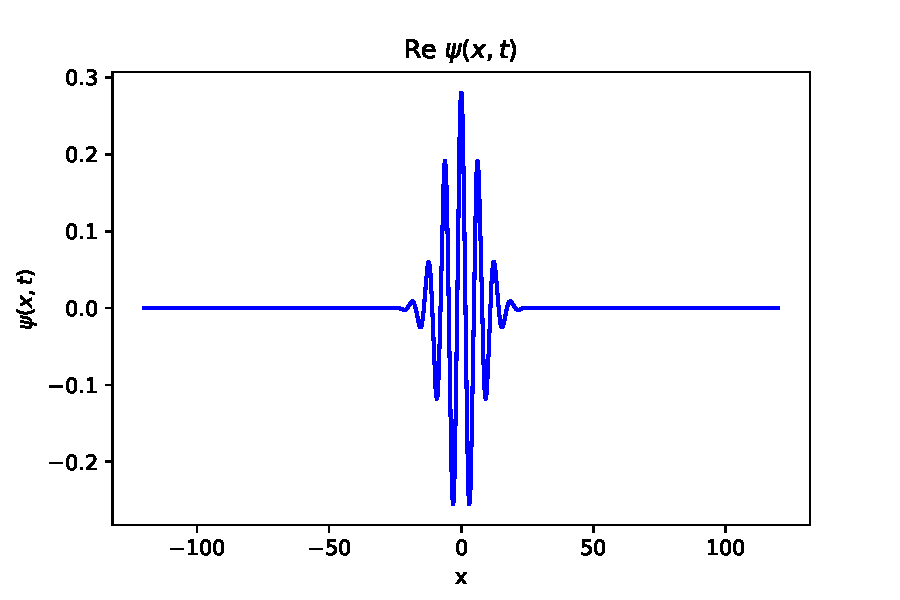
\includegraphics{images/PsiFunctionReal.pdf}
        \caption{Волновая функция. Действительная часть}
        \label{fig:PsiFunctionReal}
    \end{figure}

    \begin{figure}[h!]
        \centering
        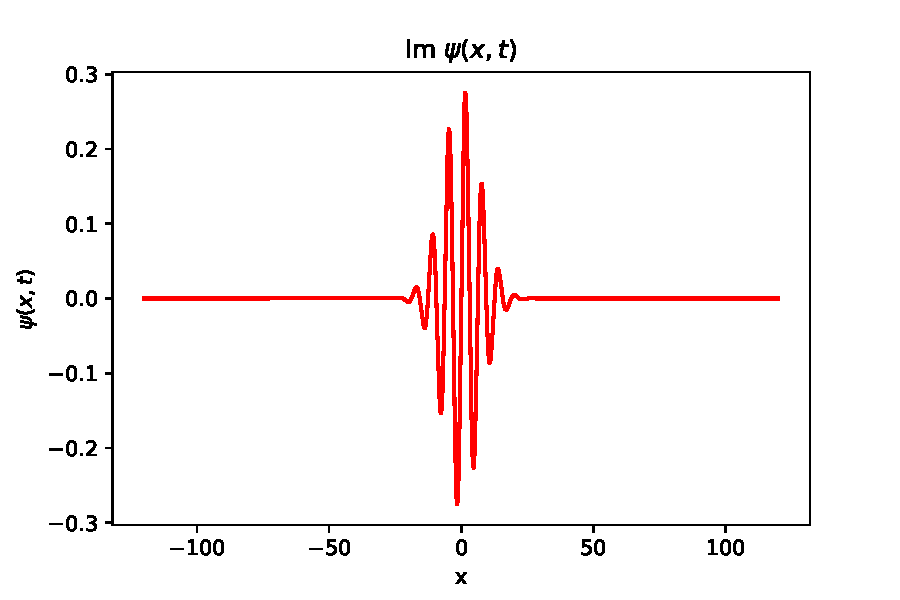
\includegraphics{images/PsiFunctionImag.pdf}
        \caption{Волновая функция. Мнимая часть}
        \label{fig:PsiFunctionImag}
    \end{figure}

    \begin{figure}[h!]
        \centering
        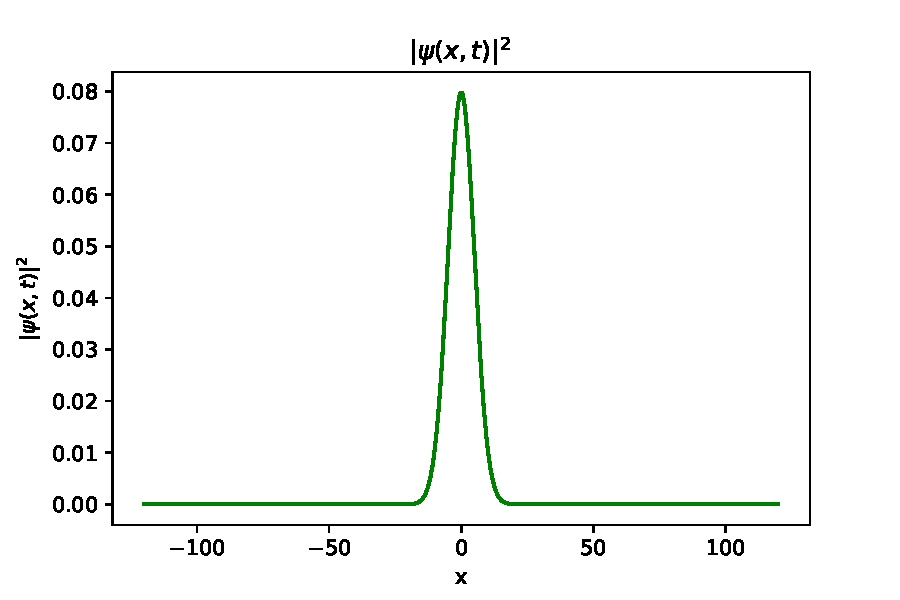
\includegraphics{images/PsiFunctionPropability.pdf}
        \caption{Модуль квадрата волновой функции}
        \label{fig:PsiFunctionPropability}
    \end{figure}

    Результат работы мы можем видеть на рисунках \ref{fig:PsiFunctionReal}, \ref{fig:PsiFunctionImag} и 
    \ref{fig:PsiFunctionPropability}. Изменение положения волновой функции со временем мы можем видеть на рисунках 
    \ref{fig:PsiTimeEvolution}, \ref{fig:PsiTimeEvolutionPropability}.

    \begin{figure}[h!]
        \centering
        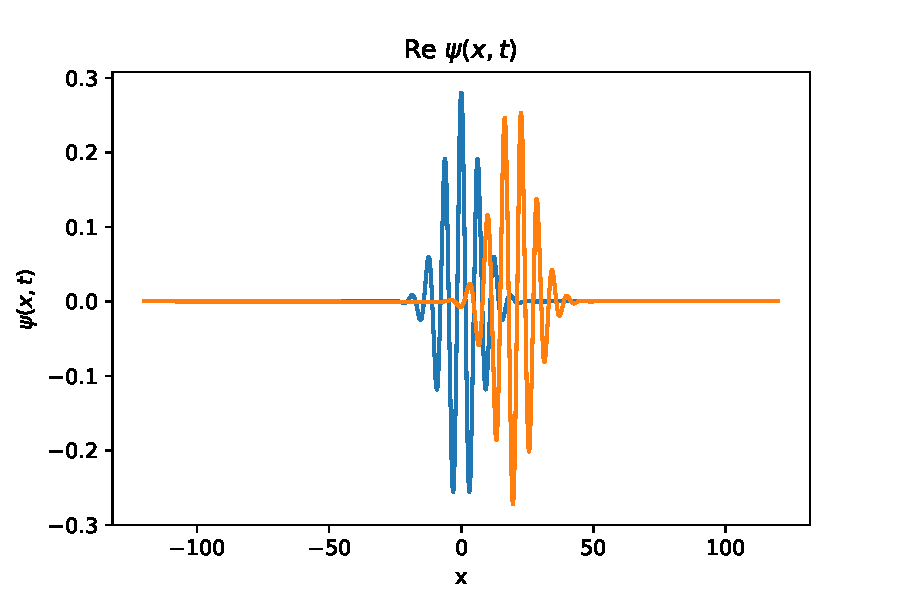
\includegraphics{images/PsiTimeEvolution.pdf}
        \caption{Изменение положения волновой функции}
        \label{fig:PsiTimeEvolution}
    \end{figure}

    \begin{figure}[h!]
        \centering
        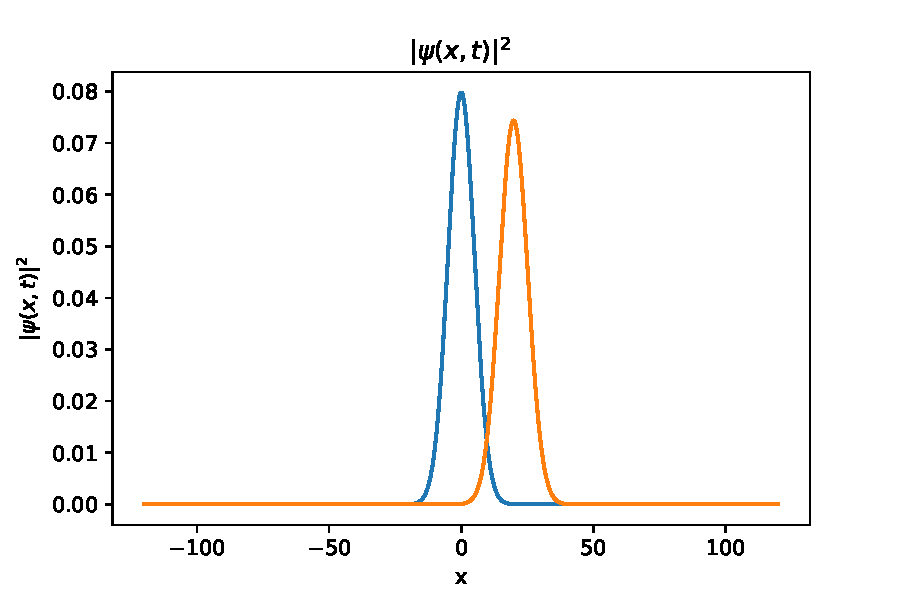
\includegraphics{images/PsiTimeEvolutionPropability.pdf}
        \caption{Изменение положения волновой функции}
        \label{fig:PsiTimeEvolutionPropability}
    \end{figure}

    \subsection{Средний импульс и средняя координата}

    Зная значение волновой функции $\psi(x, t)$ в любой точке в любой момент времени, мы сможем расчитывать средние величины
    по формуле 

    \begin{equation}
        \langle f \rangle = \int \psi^* \hat{f} \psi dV
    \end{equation}

    Заметим, что в данном случае в левой части равенства $f$ -- некоторая функция, а в правой части равенства $\hat{f}$ -- 
    \textbf{оператор}. Вспомним, что оператор импульса имеет выражение

    \begin{equation}
        \hat{p} = -i \hbar \nabla = -i \hbar \frac{\partial}{\partial x}
    \end{equation}

    Тогда мы сможем находить находить значения средней координаты и среднего импульса динамически

    \begin{equation}
        \langle x \rangle = \int \psi^* x \psi dx
    \end{equation}

    \begin{equation}
        \langle p \rangle = \int \psi^* \frac{\partial \psi}{\partial x} dx
    \end{equation}

    \subsection{Волновая функция $\psi(x, 0)$}

    Как видно из \eqref{eq:solution}, для того, чтобы построить решение, необходимо задать функцию $\psi(r, 0)$. То есть,
    задать волновую функцию в пространстве в начальный момент времени. 

    Решением стационарного уравнения Шрёдингера в общем случае является функция

    \begin{equation}
        \psi(r) = \psi_0 \exp{\frac{i \vec{p} \vec{r}}{\hbar}}
    \end{equation}

    В одномерном случае это выражение запишется в несколько упрощенном виде

    \[ \psi(r) = \psi_0 e^{\frac{i p x}{\hbar}} \]

    где $p = \sqrt{2mE}$.

    В программе в качестве начального решения будем задавать волновую функцию следующего вида

    \begin{equation}
        \psi(x) = \left(\frac{1}{\pi \sigma_0^2} \right)^{\frac{1}{4}} \exp{\left(ip_0 x - \frac{(x - x_0)^2}{2 \sigma_0^2} \right)}
    \end{equation}

    где $p_0$ -- начальный импульс, $x_0$ -- начальная координата, $\sigma_0$ -- неопределенность координаты
    (учет соотношения неопределенности).

    При этом ширина $\sigma$ не остается постоянной. Имеет место \textbf{расплывание} ширины $\sigma$ по следующему
    закону

    \begin{equation}
        \sigma(t) = \sigma_0 \sqrt{1 + \left(\frac{\hbar t}{m \sigma_0^2} \right)^2}
    \end{equation}

    \section{Краткое описание моделей}

    \subsection{Волновая функция в отсутствии препятствий}

    \begin{figure}
        \centering
        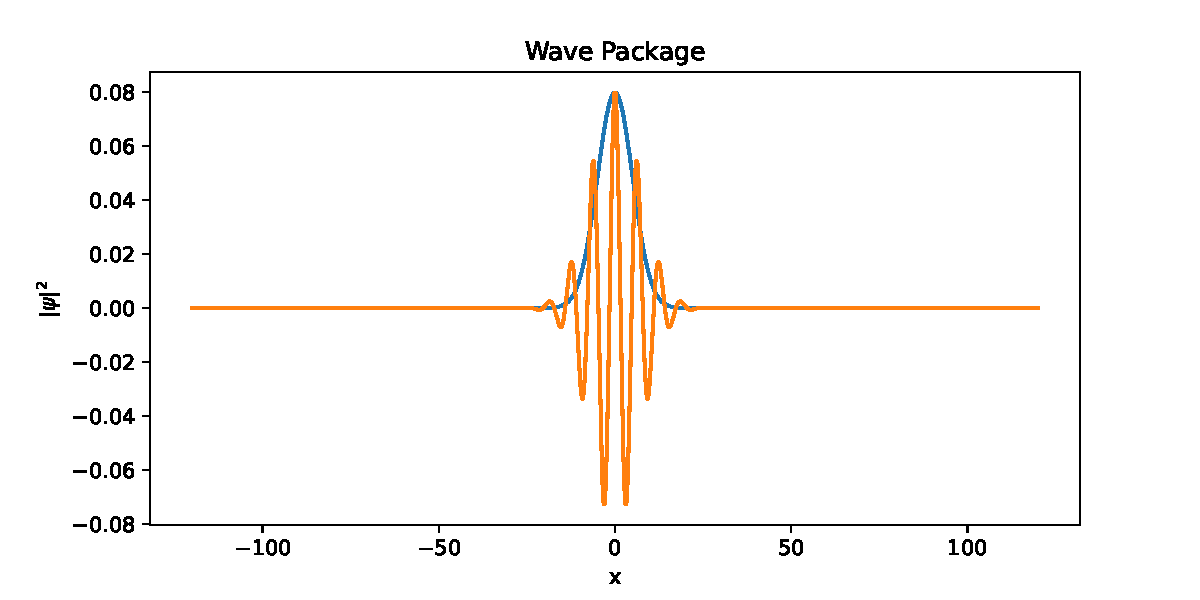
\includegraphics[scale=0.5]{images/WavePackage.pdf}
        \caption{Волновая функция в отсутствии препятствий}
        \label{fig:WavePackage}
    \end{figure}

    На примере этой модели (рис \ref{fig:WavePackage}) мы рассматриваем волновую функцию в отсутствии потенциальных барьеров. То 
    есть эта ситуация по-сути демонстрирует свободное равномерное прямолинейное движение квантовой частицы. 

    Наиболее хорошо на примере этой модели можно пронаблюдать увелиение ширины $\sigma$ с течением времени.
    Особо стоит обратить внимание на то, что чем меньше начальная ширина, тем быстрее она возрастает.
    
    \subsection{Прямоугольная потенциальная яма}

    \begin{figure}
        \centering
        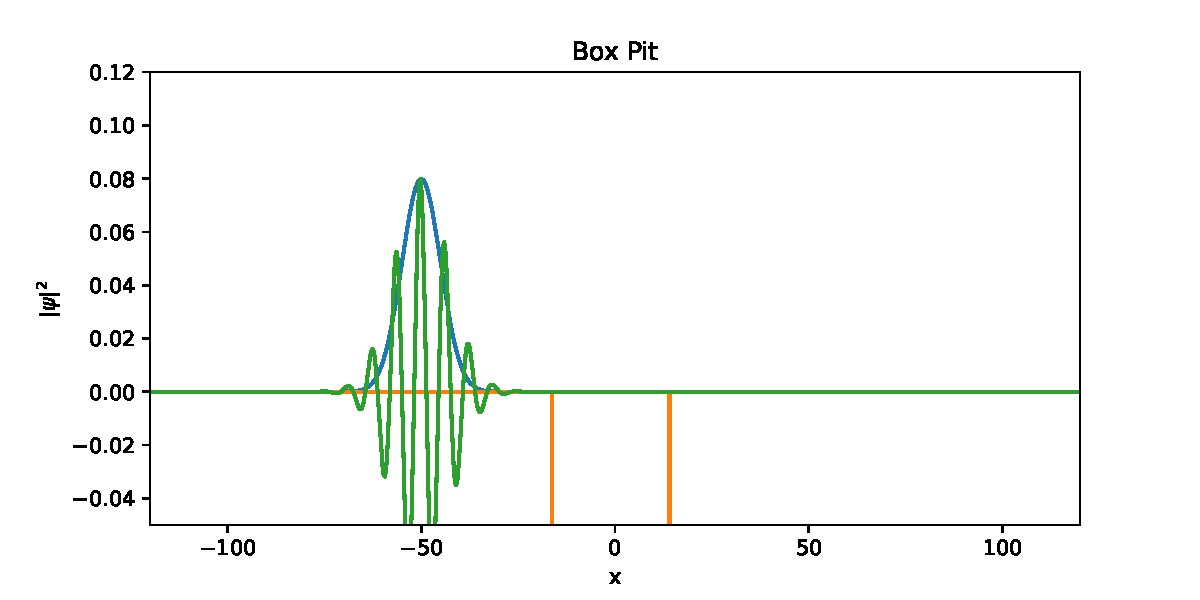
\includegraphics[scale=0.5]{images/BoxPit.pdf}
        \caption{Прямоугольная потенциальная яма}
        \label{fig:BoxPit}
    \end{figure}

    Классическая задача, рассматриваемая в курсе физики рис \ref{fig:BoxPit}. Прохождение волновой функции через потенциальню яму.
    На примере этой модели можно рассмотреть отражение и прохождение волны на границах областей.
    
    \subsection{Параболическая потенциальная яма}

    \begin{figure}
        \centering
        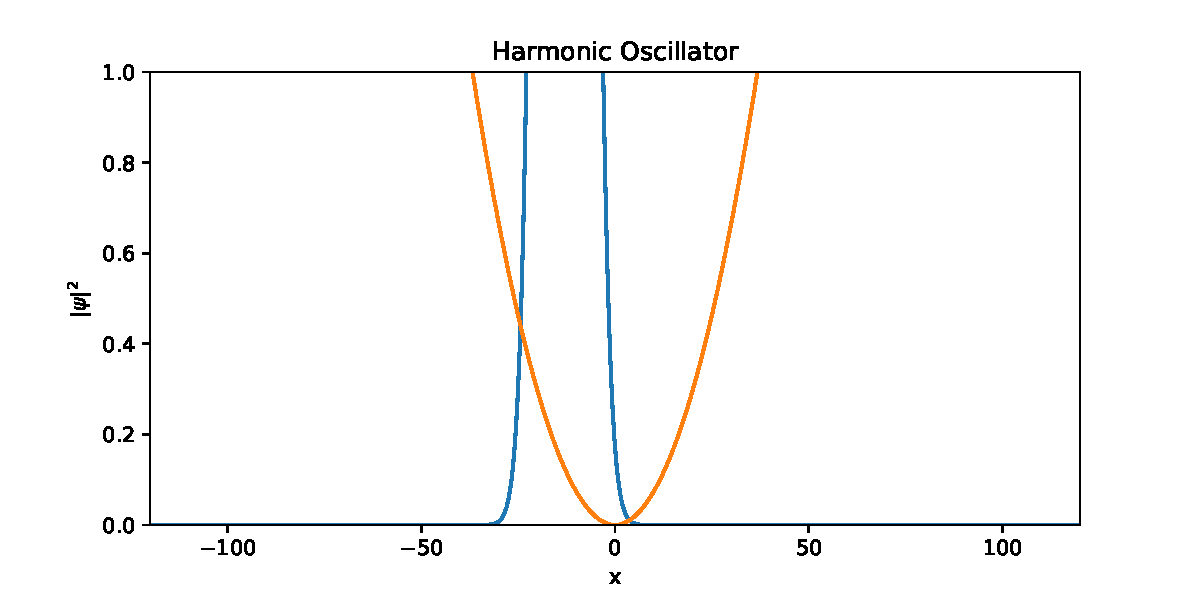
\includegraphics[scale=0.5]{images/HarmonicOscillator.pdf}
        \caption{Параболическая потенциальная яма}
        \label{fig:HarmonicOscillator}
    \end{figure}

    Модель демонстрирует осциляцию волновой функции внутри параболической потенциальной ямы 
    $\displaystyle U = \frac{a  x^2}{2}$ рис \ref{fig:HarmonicOscillator}.
    
    \subsection{Прямоугольный потенциальный барьер конечной ширины}

    \begin{figure}
        \centering
        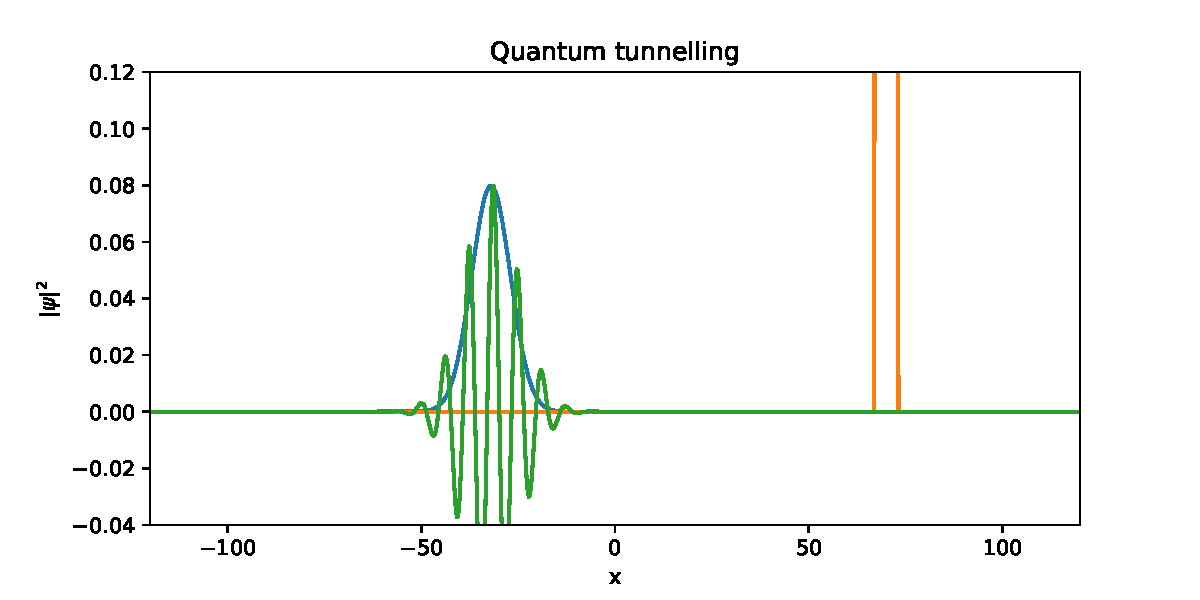
\includegraphics[scale=0.5]{images/QuantumTunnelling.pdf}
        \caption{Прямоугольный потенциальный барьер конечной ширины}
        \label{fig:QuantumTunnelling}
    \end{figure}

    Основная задача данной работы рис \ref{fig:QuantumTunnelling}. На примере модели можно рассматривать надбарьерное
    прохождение а так же эффект квантового туннелирования. Кроме того, на примере данной можели можно наблюдать
    изменение коэффициента прохождения в зависимости от энергии $E$ в случае надбарьерного и подбарьерного перехода,
    а так же в зависимости от различных параметров.
    
    \subsection{Равномерно возрастающий потенциал}

    \begin{figure}
        \centering
        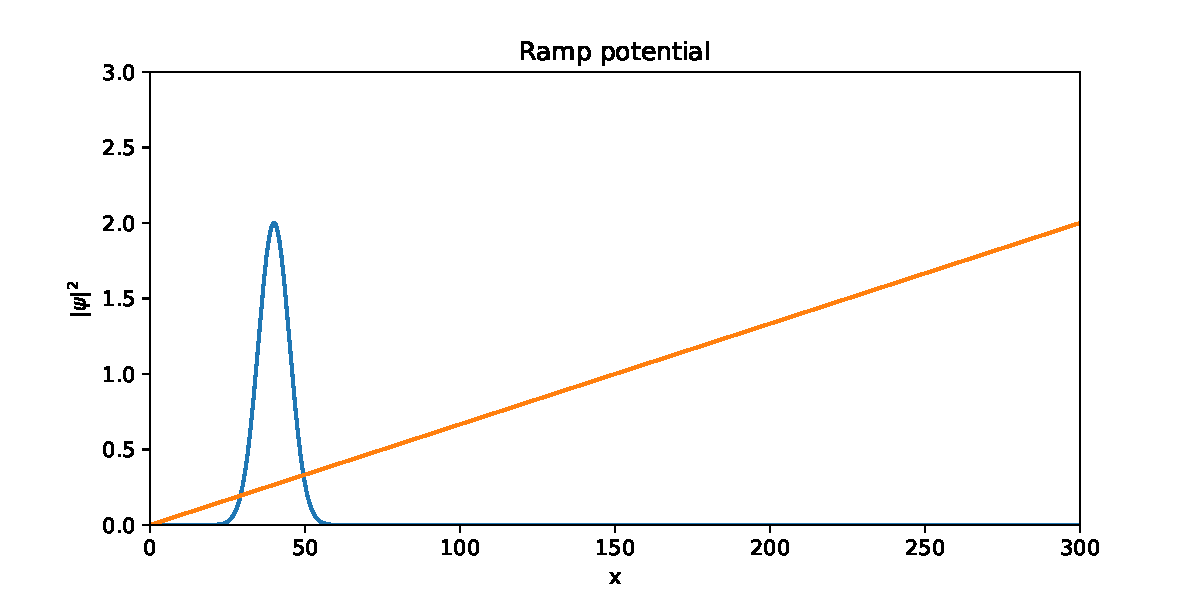
\includegraphics[scale=0.5]{images/RampPotential.pdf}
        \caption{Равномерно возрастающий потенциал}
        \label{fig:RampPotential}
    \end{figure}

    Модель демонстрирует поведение волновой функции при равномерном возрастании потенциальной энергии $U(x) = kx$ рис 
    \ref{fig:RampPotential}.
    
    \subsection{Прямоугольный потенциальный барьер}

    \begin{figure}
        \centering
        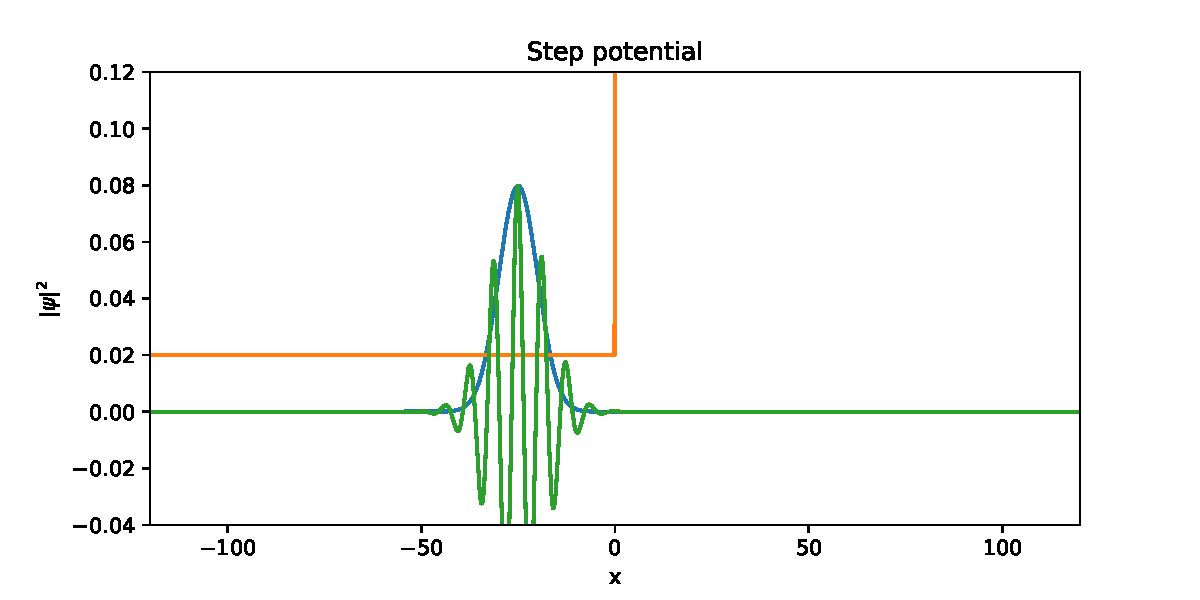
\includegraphics[scale=0.5]{images/StepPotential.pdf}
        \caption{Прямоугольный потенциальный барьер}
        \label{fig:StepPotential}
    \end{figure}

    На примере модели рассматривается проникание волновой функции под потенцильный барьер и ее экспоненциальное затухание рис 
    \ref{fig:StepPotential}.
    
    \subsection{Бесконечно глубокая потенциальная яма}

    \begin{figure}
        \centering
        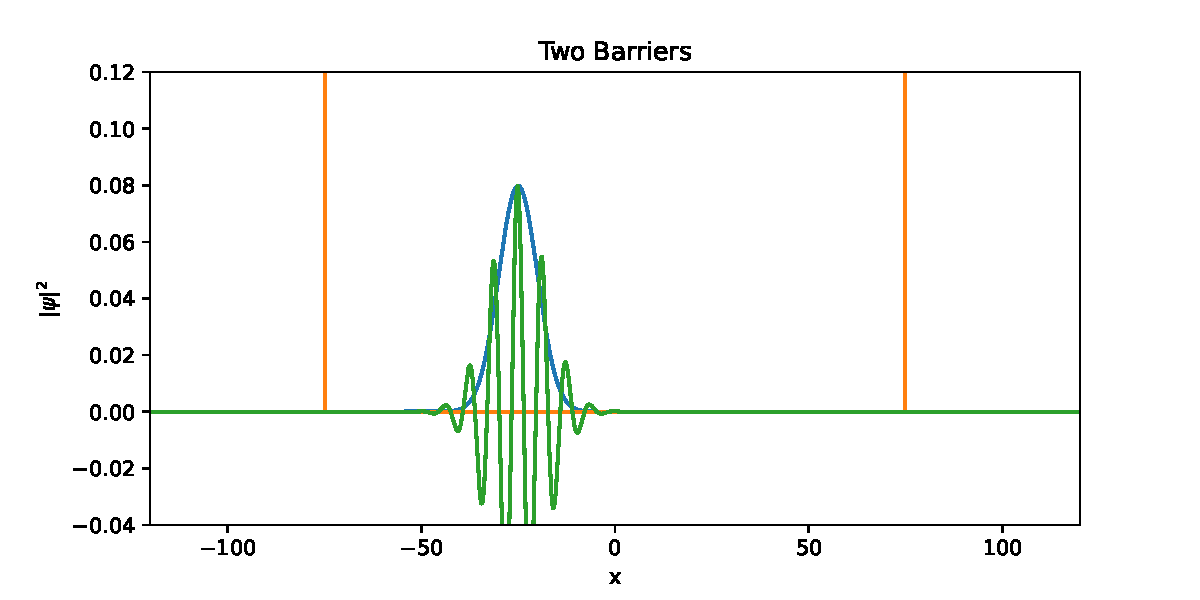
\includegraphics[scale=0.5]{images/TwoBarriers.pdf}
        \caption{Бесконечно глубокая потенциальная яма}
        \label{fig:TwoBarriers}
    \end{figure}

    Классическая задача, рассматриваемая в курсе физики -- поведение волновой функции в потенциальной яме с бесконечно высокими
    стенками \ref{fig:TwoBarriers}.
    
    \subsection{Общий случай прямоугольного потенциального барьера}

    \begin{figure}
        \centering
        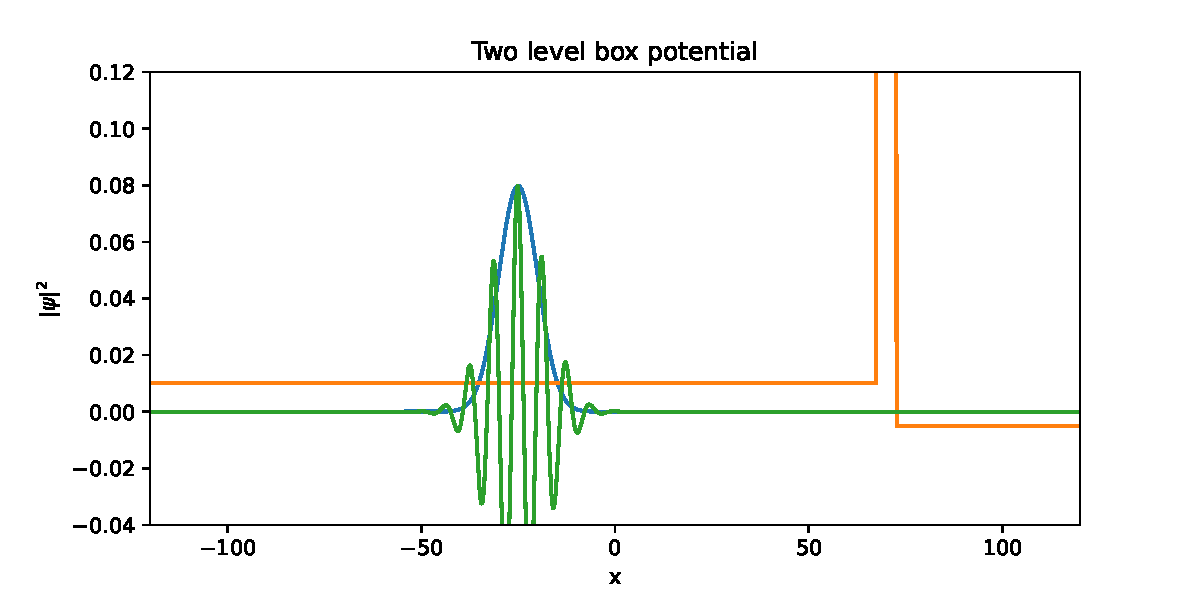
\includegraphics[scale=0.5]{images/TwoLevelBoxPotential.pdf}
        \caption{Общий случай прямоугольного потенциального барьера}
        \label{fig:TwoLevelBoxPotential}
    \end{figure}

    Чуть более общий случай ситуации, рассмотренной на рис \ref{fig:QuantumTunnelling} представлен на рис 
    \ref{fig:TwoLevelBoxPotential}. В данной модели помимо всего прочего значения потенциалов в первой и третьей областях не равны.

    \section{Вывод}

    Основной целью данно работы являлось теоретическое рассмотрение физических явлений, а так же визуальное наблюдение
    теоретических зависимостей на примере созданных качественных моделей. В данной работе при рассмотрении визуальных моделей
    мы пронаблюдали следующее:

    \begin{enumerate}
        \item Зависимость ширины волновой функции $\sigma$ от времени.
        \item Проникание волновой функции под потенциальный барьер.
        \item Надбарьерный переход.
        \item Подбарьерный переход (квантовое туннелирование).
        \item Зависимость коэффициента подбарьерного перехода от энергии $E$.
        \item Осцилирующий характер коэффициента надбарьерного перехода в зависимости от энергии $E$.
        \item Зависимость коэффициента перехода от энергии квантовой частицы $E$, высоты потенциального барьера $U$ и ширины 
        потенциального барьера $a$.
    \end{enumerate}
    
\end{document}